\documentclass{article}


\usepackage{parskip,wrapfig,graphicx}
\usepackage{hyperref}
\usepackage{fullpage}

\hypersetup{
    colorlinks,
    citecolor=black,
    filecolor=black,
    linkcolor=black,
    urlcolor=black
}




\title{Curta Type 3DP Build Manual}
\date{}

\begin{document}
\maketitle

\tableofcontents

\newpage

\section{Introduction}
This build manual is an attempt to describe the detailed and extensively manual process by which
I build my 3D printed Curta Calculators.


\section{Change Log}

\section{Safety Warning}


\section{Tools and Parts}

\section{A Note About Fitting Parts}

\section{Preparing and Painting External Facing Parts}


\section{Preparing Main Casting and Bearing Plate}
\subsection{Parts Required}

\subsection{Tools Required}

\subsection{Process}

\subsubsection{Bearing Plate Diagram (from the bottom side)}



\newpage
\section{Step Drum and Bearing Plate}

\subsection{Parts Required}

\begin{table}[h!]
 \centering
 \begin{tabular}{clc}
    Part Number & Part Name & Quantity (if $>1$) \\ \hline
     13 & Step Drum Lower or Step Drum (with main axle) & \\
     45 & Step Drum Upper Or Main Axle Bottom & \\
     78 & Step Drum Pins & 3 \\
     49 & Anti-Rotation plate (called Anti-Reversal in BoM) & \\
     33 & Tens Bell & 
 \end{tabular}
\end{table}

\subsection{Tools Required}

\begin{itemize}
 \item Hex driver or screwdriver (depending on the type of bolts you have)
 \item PTFE spray lubricant
 \item Files
 \item Sandpaper
 \item Superglue (cyanoacrylic)
\end{itemize}




\subsection{Process}
If you opted for printing the step drum as one piece, fit the main axle bottom into the base of the
step drum. This should be a snug fit with the keys matching up inside the step drum preventing any
rotation of the bottom of the axle relative to the step drum.


\begin{wrapfigure}{r}{.45\textwidth}
 \centering
 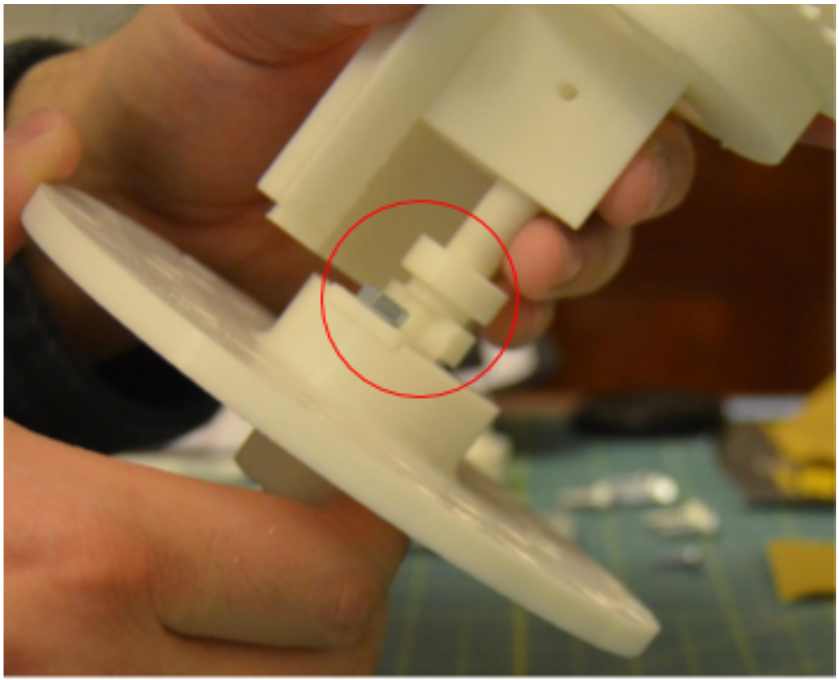
\includegraphics[width=.4\textwidth]{images/anti-rotation-collar.png}
 \caption{Alignment of the anti-rotation collar to the step drum}
\end{wrapfigure}

If you opted for printing the step drum in two pieces, fit the three pins into the lower piece of 
the step drum and super them into place. Once that has dried, add super glue to the pins of the lower
step drum and pres the upper half of the step drum onto the pins to combine the upper and lower
portions of the step drum into one piece.




The flat portion of the anti-rotation collar on the base of the axle needs to align with the right
side of the step drum when the toothed face of the step drum is facing you. This ensures that
the Curta will not switch between addition and subtraction when it is mid-rotation.



Now slide the step drum into the center of the bearing plate. The step drum should spin smoothly.
If it does not, file and sand it down until it does. Use some PTFE spray lubricant on the shaft and
the bearing plate. Do not allow the lubricant to reach the teeth of the step drum, but do allow it
to cover the anti-rotation collar. The fit should allow the step drum to spin freely. If you have to
sand further after spraying the lubricant, you will need to respray the parts that have already been
sanded.

Place the anti-rotation plate on the recessed portion of the bearing plate near the center. Turn the
step drum until the anti-rotation plate aligns with the collar and then slide the anti-rotation
plate to meet the flat portion of the anti-rotation collar. Test this fit to check that the plate
fits in the slots in the collar and that the step drum still moves freely. Sand and file as necessary
to make that happen. The step drum may need to slide up or down to align the plate with the middle 
section of the collar to get it in the correct position.

Now use a 10mm M5 bolt to secure the anti-rotation plate ensuring that it stays press against the
ant-rotation collar. If you need to, you can put a driver through the hole at the top of the step
drum to reach the bolt. I used plier for this since I had a hex bolt. \textbf{Do not over tighten
any of the screws or nuts in this build. If you strip the plastic the part will need to be reprinted}.
Fasteners should be tight, but don't crank down too much. If it will not stay as secure as you need,
use removeable threadlock.

Finally, double-check that you can still rotate the step drum smoothly and that the step drum can
switch between the raised (subtraction) position and the lowered (addition) position easily. If not,
you may need to file the anti-rotation plate or the collar some more and re-lubricate.


\end{document}






























